\chapter[Capturing Charge and Size Effects of Ions at the Graphene - Electrolyte Interface Using Polarizable Force Field Simulations]{Capturing Charge and Size Effects of Ions at the Graphene - Electrolyte Interface Using Polarizable Force Field Simulations \protect\footnote[4]{This chapter has been published as \textbf{H., Hemanth}, Mewada, R. and Mallajosyula*, S.S.; Capturing Charge and Size Effects of Ions at the Graphene - Electrolyte Interface Using Polarizable Force Field Simulations; {\textit{Nanoscale Adv.}, 2023, \textbf{5}, 796 - 804}}}
\section{Introduction}
Graphene, a 2D allotrope of carbon with a hexagonal unit cell and layered architecture has attracted significant attention from the scientific community with applications in varied fields such as desalination,\supercite{sun_selective_2014,joshi_precise_2014,homaeigohar_graphene_2017,boretti_outlook_2018,yang_ultrathin_2017} energy storage\supercite{liang_graphene-based_2009,wang_supercapacitor_2009,wang_sngraphene_2009,stoller_graphene-based_2008} and electrochemical sensing.\supercite{sheng_electrochemical_2012,pumera_graphene_2010,pumera_electrochemistry_2009} For example, by tuning the interlayer separation in graphene-oxide (GO) membranes Abraham et al. achieved near-perfect salt-rejection, establishing the applicability of graphene and graphene-oxide based membranes for desalination.\supercite{abraham_tunable_2017,nair_unimpeded_2012} For technological advancement in these applications, it is important to understand the adsorption behaviour of the constituent ions at the electrolyte - graphene interface. It is to be noted that simple theories based on the continuum model, which consider only the size and the magnitude of the charge, cannot capture the dynamics of the ion - surface interactions. The shortcomings of the continuum model are even more pronounced for hydrophobic surfaces as observed in graphene and GO sheets, where the interactions are not purely electrostatic.\supercite{mennucci_polarizable_2002} Experimental studies using deep UV second harmonic generation measurements found that direct ion - graphene interactions were responsible for the adsorption of SCN\textsuperscript{-} ions on the graphene surface, with the interactions being enthalpically driven.\supercite{mccaffrey_mechanism_2017} A simple continuum model fails to capture these effects. It has been noted that the adsorption of ions on hydrophobic surfaces is affected by various properties of the ions, including their size, polarizability and hydration free energy to name a few.\supercite{iamprasertkun_capacitance_2019,glendening_dicationwater_1996} Gaining molecular insight into the governing mechanisms of ion-adsorption requires accurate modelling of the electrolyte - graphene interface.

QM calculations can accurately predict such properties, but the scaling of O(\textit{N\textsuperscript{3-4}}) for DFT calculations limits the applicability of such methods to very small systems.\supercite{mu_hydrated_2021} In one such study the interaction of hydrated cation clusters (cation-(H\textsubscript{2}O)\textsubscript{7}) with a graphene sheet was studied which revealed reorganization of the hydration shell around K\textsuperscript{+}, allowing K\textsuperscript{+} to directly interact with the graphene sheet, while such reorganization of the hydration shell was not observed for Li\textsuperscript{+}.\supercite{mu_hydrated_2021} These static QM calculations were followed by very short (10 ps) AIMD simulations to comment on the hydration dynamics.\supercite{mu_hydrated_2021,li_unraveling_2015} These studies highlight the need for alternative methods to accurately capture the ion - graphene interaction in aqueous environments.

Molecular dynamics (MD) simulations offer a viable solution to such problems. However, MD simulations based on classical additive force fields (FFs) cannot capture the ion - graphene interactions as they do not account for charge transfer. Gas-phase and polarizable continuum model (PCM) calculations have shown that the polarizability of ions and the surface plays an important role in describing the strength and evolution of the ion - graphene interactions.\supercite{sunner_ion-solvent_1981,zhou_deciphering_2020} Based on these facts efforts have been focused towards the development of FF parameters that can describe the interactions between ions and the graphene surface.\supercite{williams_effective_2017,chen_multiscale_2018} In these studies, an additional force field term is added to describe the ion - graphene interactions. The parameters are empirically tuned to reproduce the QM calculated binding energies, thus enabling additive simulations to capture the ion - graphene interactions in an otherwise non-polarizable FF simulation.\supercite{williams_effective_2017,chen_multiscale_2018} One of the major drawbacks of such implementations is that the target DFT calculations used to tune the ion - graphene interactions overemphasize the binding energetics as they are based on a mean-field description of the solvation rather than explicit solvation.

To this end polarizable simulations offer a framework for studying the evolution of ion - graphene interactions in explicit solvent, negating the need to empirically tune the FF parameters.\supercite{lin_polarizable_2018,h_polarization_2021}  In our earlier work we described the development and testing of Drude parameters to describe multilayer and monolayer graphene surfaces.\supercite{h_polarization_2021,h_capturing_2022} Here, we study the energetics and dynamics of an aqueous salt solution - multilayer graphene system using Drude polarizable FF simulations, to critically evaluate the ability of FF parameters in describing the interfacial phenomenon.

\section{Computational Methodology}
Multilayer graphene comprising four graphene sheets with a radius of 15 $\angstrom$ and combined height of 10.04 $\angstrom$, where height corresponds to the distance between the lower graphene sheet and the top-most graphene sheet, was modelled using the Inorganic Builder plugin available in the Visual Molecular Dynamics (VMD) package.\supercite{humphrey_vmd_1996} The graphene sheets were stacked in `ABAB` arrangement to simulate multilayer graphene. The multilayer graphene was solvated to bring the final system dimensions to (29.42 x 29.42 x 45)$\angstrom$\textsuperscript{3}. We introduced one molecule (one mole) of the salt of interest (NaCl, KCl, MgCl\textsubscript{2}, CaCl\textsubscript{2} and CsCl) to the solvated system using the AutoIonize plugin available in VMD. We present a representative image of the system setup in Figure 5.1. The Chemistry at Harvard Molecular Mechanics (CHARMM36) all-atom force field (FF) was used to describe bonded and non-bonded interactions in graphene sheets and ions.\supercite{vanommeslaeghe_charmm_2009} A TIP3P three-point water model\supercite{jorgensen_comparison_1983} was used to describe water molecules in additive FF simulations.

We employed in-house scripts to add Drude particles to the final systems to generate the corresponding Drude FF files. The classical Drude oscillator polarizable FF hereto referred to as the Drude polarizable FF was used to describe non-bonded interactions in ions.\supercite{lin_polarizable_2018,h_polarization_2021} Drude polarizable FF parameters previously tested by us were used to describe bonded and non-bonded interactions in graphene sheets.\supercite{h_polarization_2021} The SWM4-NDP polarizable water model\supercite{lamoureux_polarizable_2006} was used to describe water molecules in Drude polarizable FF simulations. We restrained the bond lengths and bond angles in water molecules using the SETTLE algorithm\supercite{miyamoto_settle_1992} in Drude polarizable FF simulations.

Molecular dynamics simulations were performed using the Nanoscale Molecular Dynamics (NAMD) package\supercite{phillips_scalable_2005,phillips_scalable_2020} in an isobaric-isothermal (NPT) ensemble. Particle mesh Ewald\supercite{darden_particle_1993} (PME) summation was used to evaluate the electrostatic interactions with a real-space cut-off of 9 $\angstrom$. All simulations were performed under NTP conditions (298 K and 1 atm pressure) with Langevin dynamics and the Nos\'{e}-Hoover Langevin piston to maintain the NTP conditions. We employed an additional dual thermostat at 1 K to maintain the Drude particles at 1 K during Drude polarizable FF simulations. All systems were minimized for 4000 steps and equilibrated for 1 ns in NPT and 1 ns in NVT ensembles respectively. The central atom of the graphene sheet was restrained using a harmonic potential of 1 kcal mol\textsuperscript{-1} $\angstrom$\textsuperscript{-2} to arrest the sliding motion of the graphene sheets. No additional restraints were employed during the simulations, and the sheets were allowed to relax and breathe during the simulations. We had previously shown that constraining the graphene surface affects the energetics of the system.\supercite{h_polarization_2021} The equations of motion were integrated using a time step of 1 fs in additive FF simulations and 0.5 fs in Drude polarizable FF simulations. Production simulations were performed for a total of 100 ns for each of the six salt - graphene systems considered.

We performed simulations using adaptive biasing force (ABF) to estimate the binding free energies for ion - graphene interactions. ABF scans were performed in a window spanning 3 $\angstrom$ to 15 $\angstrom$ above the topmost graphene sheet. A biasing force of 0.20 kcal mol\textsuperscript{-1} $\angstrom$\textsuperscript{-2} was employed at both ends of the scan length. The scan window was divided into bins of 0.05 $\angstrom$ length. The ABF runs were performed in a hexagonal cell of dimensions (29.42 x 29.42 x 45) $\angstrom$\textsuperscript{3}. ABF runs were performed for a total of 100 ns, and the runs were deemed convergent when the number of observations in each bin was >1.5 x 10\textsuperscript{6}. The methodology for the calculation of ABF was adopted from the work by Comer et al.\supercite{comer_predicting_2015,poblete_determinants_2017}

The densities of ions and water at the graphene - ion interfaces were calculated using in-house scripts. Densities were computed in a window spanning 15 $\angstrom$ from the surface of the multilayer graphene. The calculation window was divided into bins of 0.1 $\angstrom$ length, and the number of observations in each bin was computed. 

% Instantaneous dipole moments for the ions were computed from the simulation trajectory using in-house codes. We calculated the vibration of the Drude particles associated with each ion over the entire simulation trajectory, and the dipole moment for each ion-Drude particle pair was computed as the vector sum of the charge of the particles (ion and the Drude particle) times the distance towards the particle from the combined center of mass of the ion-Drude particle system. The dipole moments are computed in local coordinate frames, such that the center of mass of the ion - Drude particle system is placed at origin. 

% Average dipole moments for the patches of graphene surface interacting with the ions were computed using in-house codes. Similar to the calculation of the dipole moments associated with the ions, we first iterated over all the ions present in the system, and for each ion, a cylindrical selection of carbon atoms was made, with the radius of the cylinder set to 4 $\angstrom$ and the height of the cylinder set to 14 $\angstrom$. This initial selection was then post-processed to remove water molecules and other ions that might be present, to generate the patch of graphene surface directly interacting with the ion. The dipole moment for the graphene patch was then computed as a vector sum of the charge of the particles (carbon atomand the associated Drude particle) times the distance towards the particle from the combined center of mass of the carbon atom - Drude particle system. It is important to note that the vector sum is calculated over all the carbon atoms present in the patch, with the coordinate frame shifted to each carbon atom in sequence.

\section{Results and Discussions}
\begin{figure}
    \centering
    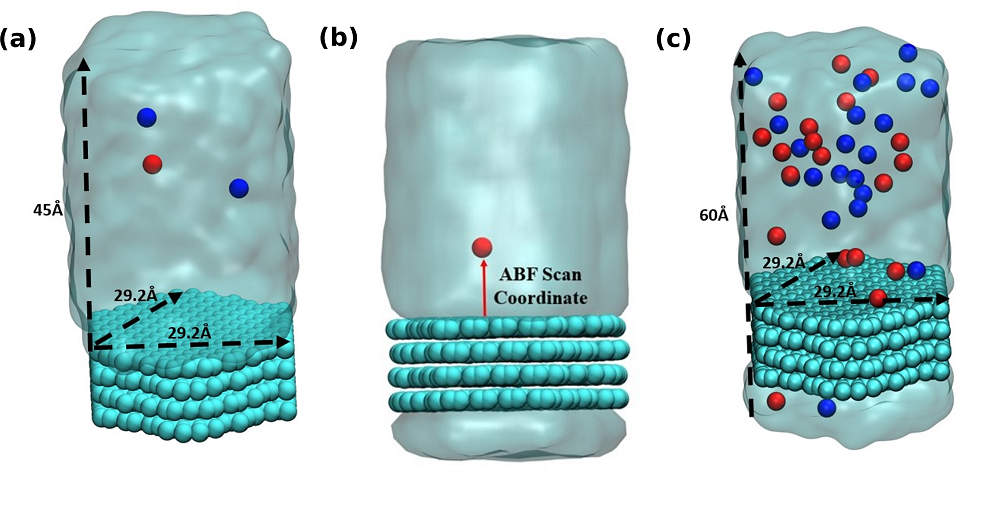
\includegraphics[width=\textwidth]{Chapter3/Figures/FigureS1.png}
    \caption[Representative structures depicting system setup for various systems investigated in this study]{(a) Representative structure depicting system setup for ABF simulations, (b) Scan coordinate used in ABF simulations, and (c) Representative structure for 1M salt solution runs. Lattice vectors for the multilayer graphene are indicated.All figures are prepared using VMD\supercite{humphrey_vmd_1996}.}
\end{figure}

Before discussing the characteristics of the ion - graphene interactions at the graphene - solvent interface we first establish the energetics of ion - graphene interactions.  To this end, we calculate the binding free energy for Li\textsuperscript{+}, Na\textsuperscript{+}, K\textsuperscript{+}, Cs\textsuperscript{+}, Mg\textsuperscript{2+}, Ca\textsuperscript{2+} and Cl\textsuperscript{-} using ABF (adaptive biasing force) simulations for both polarizable and additive force fields. We chose four monovalent cations (Li\textsuperscript{+}, Na\textsuperscript{+}, K\textsuperscript{+}, and Cs\textsuperscript{+}) and two divalent cations (Mg\textsuperscript{2+} and Ca\textsuperscript{2+}) to evaluate the influence of size and charge on the binding free energetics. Cl\textsuperscript{-} is used as the common counterion.  For the ABF simulations we use one molecule of the salt of interest in the solution. Representative images depicting the system setup for ABF simulations are presented in Figure 5.1(a). We employed the z-axis projection of the center-of-mass distance between the ions of interest and the top layer of the multilayer graphene as the scan coordinate. The scan coordinate used for the ABF simulations is presented in Figure 5.1(b). We present the potential of mean force (PMF) scans obtained from Drude polarizable and additive simulations for the monovalent cations in Figure 5.2 and for divalent cations and Cl\textsuperscript{-} ions in Figure 5.3. We also present the binding free energies obtained from Drude polarizable and additive FF simulations in Table 5.1. The binding free energies were estimated with respect to the minimum in the PMF scan and the well separated structure. For the monovalent ions, Li\textsuperscript{+}, Na\textsuperscript{+}, K\textsuperscript{+} and Cs\textsuperscript{+}, the binding free energies from Drude polarizable (additive) FF simulations are estimated to be -6.91 (-7.84), -5.83 (-1.10), -7.13 (-0.56) and -13.26 (-5.38). All energies are reported in kJ mol\textsuperscript{-1}. In Table 5.1 we also report the difference ($\Delta$E\textsubscript{1}) between the Drude polarizable and the additive binding energies. $\Delta$E\textsubscript{1} for Li\textsuperscript{+}, Na\textsuperscript{+}, K\textsuperscript{+} and Cs\textsuperscript{+} is observed to be 0.93 kJ mol\textsuperscript{-1}, -4.73 kJ mol\textsuperscript{-1}, -6.57 kJ mol\textsuperscript{-1} and -7.88 kJ mol\textsuperscript{-1} respectively.  We observe that except for Li\textsuperscript{+} the binding free energies estimated from Drude polarizable simulations are higher than the corresponding values obtained from the additive simulations. This indicates a stronger binding between the graphene surface and the monovalent ions in Drude polarizable simulations when compared to the additive simulations.  Earlier efforts to study ion - graphene interactions using MD simulations relied on capturing DFT derived binding profiles.\supercite{williams_effective_2017,chen_multiscale_2018} These have been found to overestimate the binding energetics.\supercite{elliott_qmmd_2020} We present a comparison of the binding free energies obtained by us with those obtained in these earlier studies to put the values obtained by us into perspective.  In Table 5.1 we present the adsorption energies estimated by Carbone et al. using CPCM DFT calculations (E\textsubscript{DFT}) and from PMF scans obtained after tuning the additive FF parameters (E\textsubscript{additive}\textsuperscript{\#}) to reproduce the CPCM DFT calculations. The E\textsubscript{additive}\textsuperscript{\#} values for Li\textsuperscript{+}, Na\textsuperscript{+} and K\textsuperscript{+} were reported to be -10.7 kJ mol\textsuperscript{-1}, -14.5 kJ mol\textsuperscript{-1} and -12.3 kJ mol\textsuperscript{-1}. The values obtained by us using the Drude polarizable FF are lower than those estimated by Carbone et al. In a follow up study Carbone et al. highlighted two potential shortcomings of the Lennard-Jones parameters optimized by them: (i) the model was parametrized using a single ion thereby the effect of ionic screening due to multiple ions was only included via the standard Lorentz-Berthelot combination rules and (ii) the model did not account for the polarization of the graphene surface due to the specific arrangement of the water molecules at the interface.\supercite{elliott_qmmd_2020} We note that these effects might have contributed to the very high adsorption energies observed by Carbone et al. DFT typically overestimates the adsorption of the ions onto the graphene sheet as it does not account for the screening of the charges by the water molecules. Fang et al. studied the interaction of hydrated cations, Li\textsuperscript{+}-(H\textsubscript{2}O)\textsubscript{n}, Na\textsuperscript{+}-(H\textsubscript{2}O)\textsubscript{n} and K\textsuperscript{+}-(H\textsubscript{2}O)\textsubscript{n} with the graphene sheet.\supercite{mu_hydrated_2021} The values for Li\textsuperscript{+}-(H\textsubscript{2}O), Na\textsuperscript{+}-(H\textsubscript{2}O) and K\textsuperscript{+}-(H\textsubscript{2}O) were observed to be around -42.0, -35.0 and -29.0 kcal mol\textsuperscript{-1} respectively, while the same for Li\textsuperscript{+}-(H\textsubscript{2}O)\textsubscript{9}, Na\textsuperscript{+}-(H\textsubscript{2}O)\textsubscript{9} and K\textsuperscript{+}-(H\textsubscript{2}O)\textsubscript{9} were observed to be -21.12, -22.27 and -22.98 kcal mol\textsuperscript{-1}. We clearly observe a screening effect upon the inclusion of water which is inversely correlated to the size of the cation; hence parameterizing the FF using a simple screened model would result in overstabilization.\supercite{mu_hydrated_2021} In contrast in the Drude polarizable FF the ions were parametrized to be consistent with aqueous bulk thermodynamic properties, such as hydration free energies, self-diffusion coefficients and the energetics of small ion - water clusters, thereby capturing the screening effects introduced by solvation.\supercite{yu_simulating_2010} This is also reflected in the PMF curves obtained from the Drude polarizable simulations wherein with increasing size of the monovalent cation, we observe signatures of the stabilization of the hydrated species.

\begin{table}
    \centering
    \caption[Binding free energies of ions obtained from Drude polarizable and additive FF ABF simulations. Binding energies from literature are also presented]{Binding free energies of ions obtained from Drude polarizable and additive FF ABF simulations. Binding energies are calculated as the difference between the energies of the equilibrium structure (global minimum) and the well-separated structure. $\Delta E_{1}$ is calculated using the formula $\Delta E_{1}$ = $E_{Drude}$ - $E_{additive}$. $E_{DFT}$ corresponds to the binding free energies obtained by Carbone et al. using CPCM DFT calculations.\supercite{williams_effective_2017} $E_{additive}^{\#}$ corresponds to the binding free energies obtained by Carbone et al. using modified additive FF parameters.\supercite{williams_effective_2017}  Ionic radii in solution.\supercite{marcus_ionic_1988} All energies are presented in kJ mol\textsuperscript{-1}. Radii are presented in $\angstrom$.}
    \begin{tabular}{ccccccc}
        \toprule
        Ion                     &   $E_{Drude}$ &   $E_{additive}$  &   $\Delta E_{1}$  &   $E_{DFT}$\supercite{williams_effective_2017}    &   $E_{additive}^{\#}$\supercite{williams_effective_2017}   &   Ionic Radii\supercite{marcus_ionic_1988} \\ \midrule
        Li\textsuperscript{+}   & -6.91  & -7.84 & 0.93  & -10.4 & -10.7 & 0.71 \\
        Na\textsuperscript{+}   & -5.83  & -1.10 & -4.73 & -13.8 & -14.5 & 0.97 \\
        K\textsuperscript{+}    & -7.13  & -0.56 & -6.57 & -12.6 & -12.3 & 1.41 \\
        Cs\textsuperscript{+}   & -13.26 & -5.38 & -7.88 & —     & —     & 1.73 \\
        Mg\textsuperscript{2+}  & -1.0   & -6.59 & 5.59  & -16.5 & -16.3 & 0.70 \\
        Ca\textsuperscript{2+}  & -2.93  & -1.03 & -1.9  & -15.7 & -16.3 & 1.03 \\
        Cl\textsuperscript{-}   & -5.26  & -5.76 & 0.5   & -6.90 & -7.0  & 1.80 \\ \bottomrule
    \end{tabular}
\end{table}

\begin{figure}
    \centering
    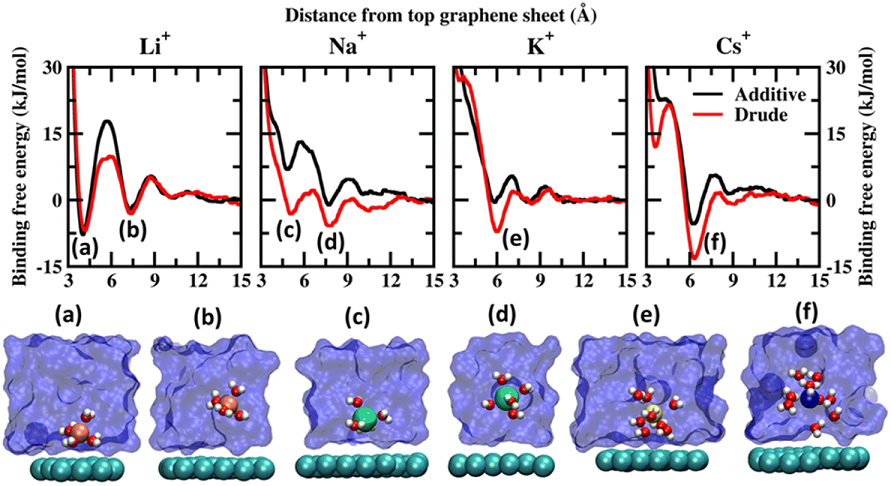
\includegraphics[width=\textwidth]{Chapter3/Figures/Figure2.png}
    \caption[Potential of mean force (PMF) obtained from additive and Drude polarizable FF simulations of monovalent cations considered in this study. Representative structures corresponding to the minima present in the PMF surface obtained from Drude polarizable simulations are also presented to highlight the different interaction modes]{Potential of mean force (PMF) obtained from additive and Drude polarizable FF simulations of monovalent cations, Li\textsuperscript{+}, Na\textsuperscript{+}, K\textsuperscript{+} and Cs\textsuperscript{+}, considered in this study. All energies are reported in units of kJ mol\textsuperscript{-1}. All distances are presented in units of $\angstrom$. Representative structures corresponding to the minima present in the PMF surface obtained from Drude polarizable simulations are presented to highlight the interaction modes. Ions, the underlying graphene sheet and water molecules in the 1\textsuperscript{st} hydration shell are presented in VdW representation. The remaining solvent molecules are presented using a solvent environment to illustrate the solvent environment. Only a small section of the sheet and the solvent are presented for clarity. All figures are prepared using VMD.\supercite{humphrey_vmd_1996}}
\end{figure}

\begin{table}
    \centering
    \small
    \caption[Location of the global minima and next minima observed in the potential energy surface obtained from Drude polarizable and additive PMF simulations]{Location of the global minima and next minima observed in the potential energy surface obtained from Drude polarizable and additive PMF simulations. All distances are presented in units of $\angstrom$.}
    \begin{tabular}{ccccc}
    \toprule
    % Ion         &   Drude Polarizable FF ($\angstrom$)  &               &   additive FF ($\angstrom$)   &                \\
    Ion         &   Minima\textsuperscript{Drude}($\angstrom$)    & Next Minima\textsuperscript{Drude}($\angstrom$)   &   Minima\textsuperscript{add.}($\angstrom$)  &   Next Minima\textsuperscript{add.}($\angstrom$)  \\ \midrule
    Li\textsuperscript{+}                           & 4.20                       & 7.40                     & 4.05                   & 7.25                 \\
    Na\textsuperscript{+}                           & 7.75                       & 5.10                     & 7.75                   & 5.10                 \\
    K\textsuperscript{+}                            & 5.95                       & —                        & 8.10                   & 5.85                 \\
    Cs\textsuperscript{+}                           & 6.35                       & —                        & 6.25                   & —                    \\
    Mg\textsuperscript{2+}                          & 7.55                       & 4.80                     & 4.75                   & 7.46                 \\
    Ca\textsuperscript{2+}                          & 5.95                       & 5.05                     & 7.75                   & 4.70                 \\
    Cl\textsuperscript{-}                           & 3.90                       & —                        & 6.10                   & —                    \\ \bottomrule
    \end{tabular}
    \end{table}

From Figure 5.2, we note that the binding energy curves for all the monovalent ions are predominantly characterized by two minima, the first one at a distance close to $\approx$4 $\angstrom$ and the other minima at a distance $\geq$6 $\angstrom$. These minima correspond to two distinct interaction modes, (i) wherein the ions interact directly with the graphene surface or as a partially solvated species and (ii) wherein the ions interact with the graphene surface through a solvation shell. The distances corresponding to the global minima and the next minima from both the Drude polarizable and additive simulations are tabulated in Table 5.2 for all the systems. For Li\textsuperscript{+}, we observe that the ions favor interacting directly with the graphene sheet at a distance of 4.20 (4.05) $\angstrom$ in Drude polarizable (additive) FF simulations, with binding free energies of -6.91 (-7.84) kJ mol\textsuperscript{-1}. The solvent separated interaction mode is observed at a distance of 7.40 (7.25) $\angstrom$ with binding free energies of -3.09 (-2.10) kJ mol\textsuperscript{-1}. For the remaining monovalent cations Na\textsuperscript{+}, K\textsuperscript{+} and Cs\textsuperscript{+} the solvent separated minima is observed to be the global minima. For Na\textsuperscript{+} ions the global minimum is observed as a solvent separated interaction at a distance of 7.75 $\angstrom$ in both the Drude polarizable and additive simulations. The binding free energy corresponding to this minimum is observed to be -5.83 kJ mol\textsuperscript{-1} and -1.1 kJ mol\textsuperscript{-1} form Drude polarizable and additive simulations respectively.  We observe that the Drude polarizable simulations also favour the direct interaction of the Na\textsuperscript{+} ions and the graphene sheet with a minimum in the binding free energy profile appearing at a distance of 5.10 $\angstrom$, with the binding free energy being -3.15 kJ mol\textsuperscript{-1}. This interaction is not favoured in the additive simulations with the binding free energy being 7.13 kJ mol\textsuperscript{-1}. With increasing size of the ionic radii of the ions we observe the stabilization of the solvent separated minima for both the K\textsuperscript{+} and Cs\textsuperscript{+} species. From the Drude polarizable simulations the minima for K\textsuperscript{+} are observed at 5.95 $\angstrom$, with the binding free energy being -7.13 kJ mol\textsuperscript{-1}. On the other hand, from the additive simulations we observe two shallow minima at 5.85 $\angstrom$ and 8.10 $\angstrom$, with the corresponding binding energy being -0.53 kJ mol\textsuperscript{-1}. For Cs\textsuperscript{+}, a single global minimum is observed at 6.35 $\angstrom$ and 6.25 $\angstrom$ for the Drude polarizable and additive simulations with the binding free energy being -13.26 kJ mol\textsuperscript{-1} and -5.38 kJ mol\textsuperscript{-1} respectively. Overall, for the monovalent ions the binding free energy follows the pattern Cs\textsuperscript{+} > K\textsuperscript{+} > Li\textsuperscript{+} > Na\textsuperscript{+} for the Drude polarizable simulations, while for the additive simulations the pattern is Li\textsuperscript{+} > Cs\textsuperscript{+} > Na\textsuperscript{+} > K\textsuperscript{+}. It can be inferred that the solvent separated interactions are stabilized in the Drude polarizable FF when compared to the additive FF, which is indicative of differential solvation dynamics observed in the Drude polarizable and the additive simulations.

\begin{figure}
    \centering
    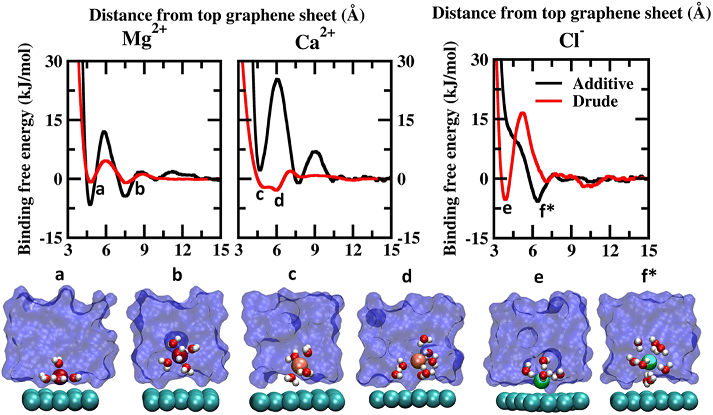
\includegraphics[width=\textwidth]{Chapter3/Figures/Figure3.png}
    \caption[Potential of mean force (PMF) obtained from additive and Drude polarizable FF simulations of divalentvalent cations and Cl\textsuperscript{-} considered in this study. Representative structures corresponding to the minima present in the PMF surface obtained from Drude polarizable simulations are also presented to highlight the interaction modes]{Potential of mean force (PMF) obtained from additive and Drude polarizable FF simulations of divalent cations, Mg\textsuperscript{2+} and Ca\textsuperscript{2+} and counter-ion Cl\textsuperscript{-}, considered in this study. All energies are reported in units of kJ mol\textsuperscript{-1}. All distances are presented in units of $\angstrom$. Representative structures corresponding to the minima present in the PMF surface obtained from Drude polarizable simulations are presented to highlight the interaction modes. Ions, the underlying graphene sheet and water molecules in the 1st hydration shell are presented in VdW representation. The remaining solvent molecules are presented using a solvent environment to illustrate the solvent environment. Only a small section of the sheet and the solvent are presented for clarity. All figures are prepared using VMD.\supercite{humphrey_vmd_1996} The representative structure corresponding to the minima present in the PMF surface obtained from additive simulations of Cl\textsuperscript{-} ions is also presented.}
\end{figure}

The PMF scans obtained from Drude polarizable and additive simulations for divalent cations and Cl\textsuperscript{-} ions are presented in Figure 5.3. For the divalent ions Mg\textsuperscript{2+} and Ca\textsuperscript{2+}, we observe interaction patterns that are consistent with the dependence of the ionic radii of these species. The ionic radii of Mg\textsuperscript{2+} (0.70 $\angstrom$) are similar to the ionic radii of Li\textsuperscript{+} (0.71 $\angstrom$). From the additive simulations we observe that similar to Li\textsuperscript{+} the Mg\textsuperscript{2+} ions favour interacting directly with the graphene sheet with the global minima appearing at 4.75 $\angstrom$. The binding free energy corresponding to this interaction is found to be -6.59 kJ mol\textsuperscript{-1}. The solvent-separated minima are observed at 7.46 $\angstrom$, with the binding free energy being -4.45 kJ mol\textsuperscript{-1}. From the Drude polarizable simulations we observe two shallow minima at 4.80 $\angstrom$ and 7.55 $\angstrom$, which correspond to the direct interaction and solvent-separated interaction of Mg\textsuperscript{2+} with the graphene surface. The binding free energy corresponding to these minima is found to be -0.85 kJ mol\textsuperscript{-1} and -1.00 kJ mol\textsuperscript{-1} respectively. We observe that for both Li\textsuperscript{+} and Mg\textsuperscript{2+} the additive FF stabilizes the direct interaction of the ions with the graphene surface when compared to the Drude polarizable FF. We notice that this is directly related to the ability of the ions to polarize their surrounding solvation shell. In the Drude polarizable FF simulations the water model captures the influence of polarization while in the additive simulations the rigid water model does not account for the change in the polarizability. This is discussed subsequently in the chapter. For Ca\textsuperscript{2+} (1.03 $\angstrom$) the behaviour is similar to the Na\textsuperscript{2+} (0.97 $\angstrom$), which share comparable ionic radii. Similar to Na\textsuperscript{+} the additive FF favours only the solvent-separated interaction between the Ca\textsuperscript{2+} ions and the graphene sheet with the global minima being observed at 7.75 $\angstrom$ and the corresponding binding free energy being -1.03 kJ mol\textsuperscript{-1}. The direct interaction of Ca\textsuperscript{2+} ions with the graphene sheet is not favoured with the free energy cost of the interaction being 2.21 kJ mol\textsuperscript{-1} for the minima appearing at 4.70 $\angstrom$. From the Drude polarizable simulations we observe a free energy distribution that is different from that of the additive simulations. Two closely spaced minima are observed at 5.05 $\angstrom$ and 5.95 $\angstrom$, with the binding free energies being -2.21 kJ mol\textsuperscript{-1} and -2.93 kJ mol\textsuperscript{-1}. This corresponds to the stabilization of the partially solvated cation interacting with the graphene surface. 

The major differences between the additive and Drude polarizable FF are observed for the chloride anions (Cl\textsuperscript{-}). From the additive simulations we observe a minimum at a distance of 6.1 $\angstrom$ from the graphene surface, with the binding free energy being -5.76 kJ mol\textsuperscript{-1}. On the other hand, from the Drude polarizable simulations we observe the minimum at a distance of 3.9 $\angstrom$ from the graphene surface, with the binding free energy being -5.26 kJ mol\textsuperscript{-1}. In the Drude polarizable simulations we observe the preference for a direct interaction between Cl\textsuperscript{-} and the graphene surface, while in additive simulations the interaction between the Cl\textsuperscript{-} ions and the graphene surface is mediated via a solvation shell. Both, experimental studies\supercite{lee_role_2020} and ab initio calculations\supercite{shi_unexpectedly_2012,liu_super-strong_2021,xiaozhen_dft_2022,kim_theoretical_2004} have shown that anions interact directly with the graphene surface. Experimental studies using deep UV second harmonic generation measurements found direct ion - graphene interactions to be responsible for the adsorption of SCN\textsuperscript{-} ions on the graphene surface, with the interactions being enthalpically driven.\supercite{mccaffrey_mechanism_2017} The free energy of adsorption of the thiocyanate to the graphene was estimated to be -8.5 ± 1.1 kJ mol\textsuperscript{-1}. The experimental studies also point towards a direct interaction between the anions and the graphene surface which is captured only by the Drude polarizable FF simulations. It was noted that the anions strongly polarize the graphene surface and the water molecules, which results in the direct interaction between the ions and the graphene surface. This behaviour was not captured by additive simulations and required the inclusion of explicit polarization in molecular dynamics simulations to capture the effect. The anion - graphene interactions have been described earlier by accounting for the polarization using a QM/MD coupling method,\supercite{elliott_qmmd_2020} force field based on a neural network model\supercite{di_pasquale_dynamically_2021} and explicitly polarizable force fields.\supercite{misra_ion_2021} Our results agree with those of earlier studies on the explicit inclusion of polarization. 

\begin{figure}
    \centering
    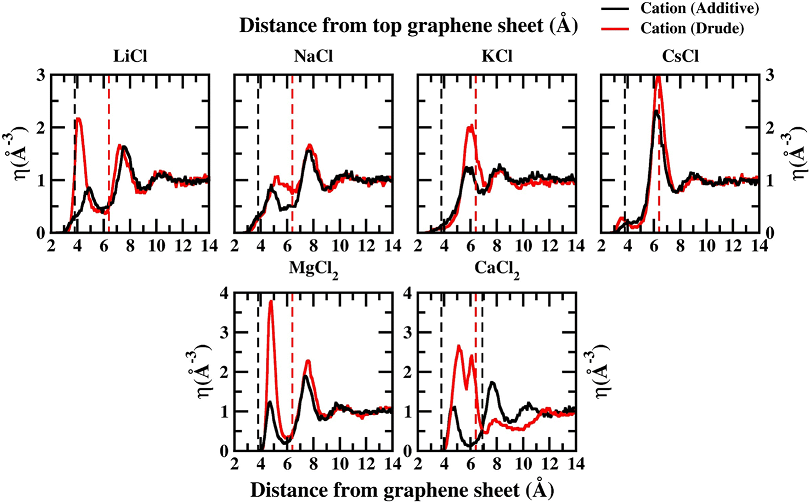
\includegraphics[width=\textwidth]{Chapter3/Figures/Figure4.png}
    \caption[Density profiles for all ions calculated from additive and Drude polarizable FF simulations of 1 M salt solutions. Location of the peak corresponding to the Cl\textsuperscript{-} ion density is depicted using dashed lines]{Density profiles for all ions calculated from additive (black) and Drude polarizable (red) FF simulations of 1 M salt solutions. In each panel we also present the location of the peak corresponding to the Cl\textsuperscript{-} ion density using dashed lines. All densities are presented in units of $\angstrom^{-3}$ and all distances are presented in units of $\angstrom$.}
\end{figure}

\begin{figure}
    \centering
    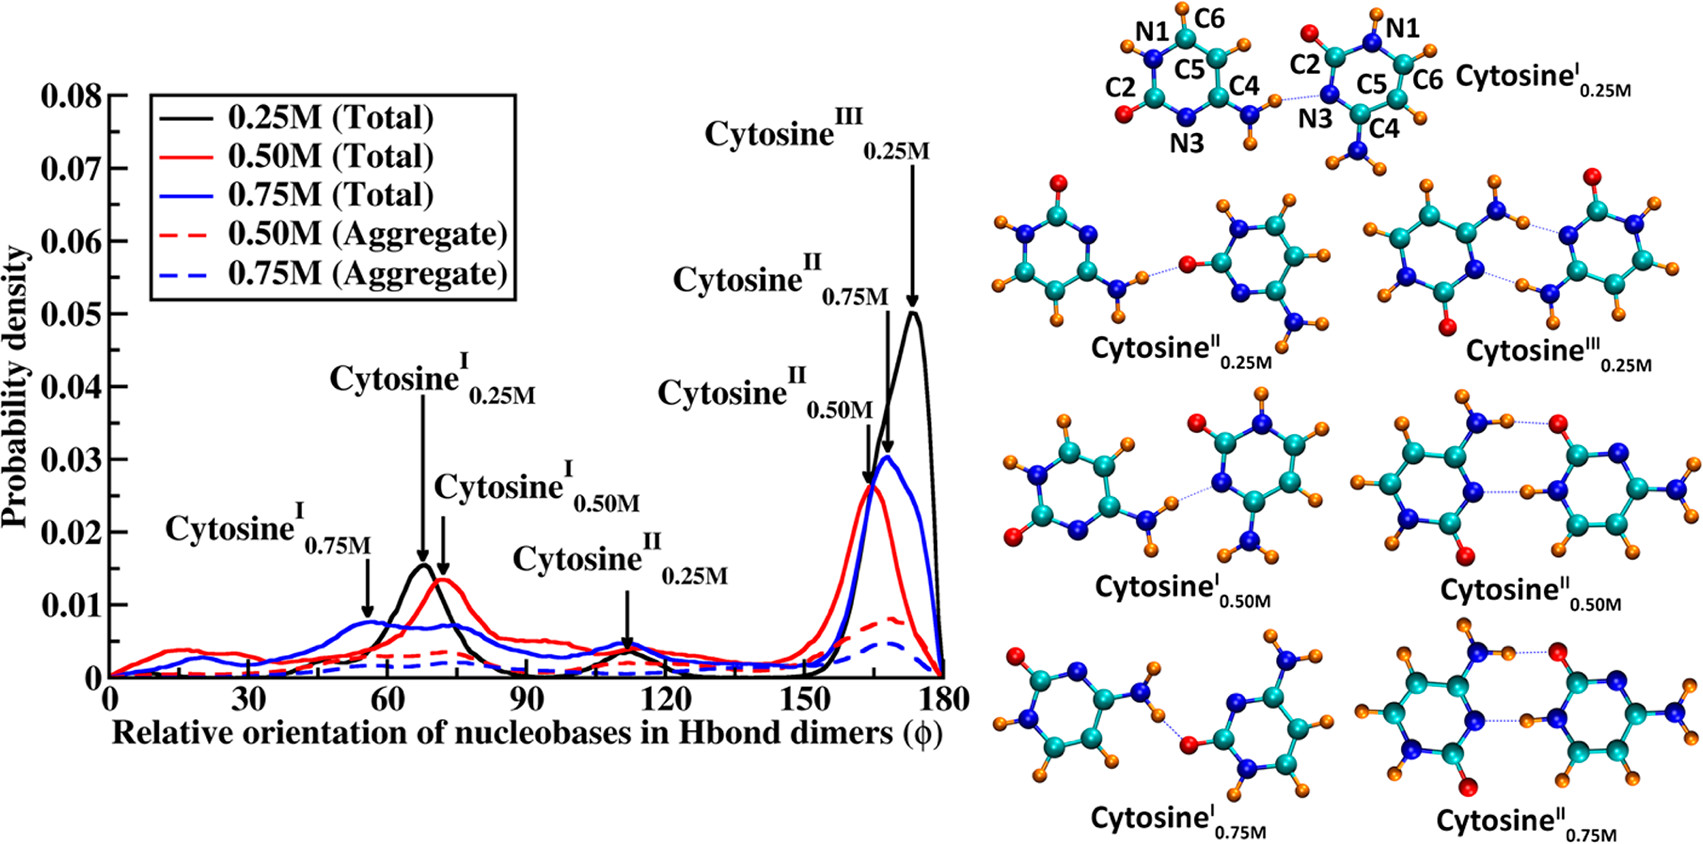
\includegraphics[width=\textwidth]{Chapter3/Figures/Figure5.png}
    \caption[Number density ($\eta$) for water molecules as a function of the distance from topmost graphene sheet, from 1M additive and Drude polarizable FF salt simulations]{Number density ($\eta$) for water molecules as a function of the distance from topmost graphene sheet, from 1M additive and Drude polarizable FF salt simulations. All distances are presented in units of $\angstrom$.}
\end{figure}

In order to capture the influence of the FF on interfacial dynamics in a realistic system we study the dynamics of 1 M salt solutions of LiCl, NaCl, KCl, CsCl, MgCl\textsubscript{2} and CaCl\textsubscript{2}. A representative image depicting the system setup is presented in Figure 5.1(c). We compute the density profiles of the ions as a function of the distance from the topmost graphene surface to establish the effect of polarization on the ion - graphene interactions. The density profiles obtained from additive and Drude polarizable FF simulations are presented in Figure 5.4. Before commenting on the distribution of the cations we analyse the distribution of the water and the counter-ion Cl\textsuperscript{-} in these simulations. The distribution of the water molecules as a function of distance from the topmost graphene sheet for all the systems is presented in Figure 5.5.  For all the systems, we observe a bimodal distribution with peaks at 3.30 $\angstrom$ and 6.10 $\angstrom$ for the TIP3P additive water model and at 3.40 $\angstrom$ and 6.20 $\angstrom$ for the SWM4 Drude polarizable water model.  The first peak corresponds to the direct interaction of the water molecules with the graphene sheet. In Figure 5.6 we present the distribution of the counterion Cl\textsuperscript{-} as a function of the distance from the topmost graphene surface for all the systems. In the additive simulations we observe a significant peak at around 6.40 $\angstrom$ for all the systems. This peak is indicative of fully solvated Cl\textsuperscript{-} ions interacting with the graphene surface in the additive simulations. For the Drude polarizable simulations we observe a significant peak at around 3.80 $\angstrom$ which implies a direct interaction between the Cl\textsuperscript{-} ions and the graphene surface. These observations are directly related to the underlying free energy distribution, wherein the free energy minimum is observed at around 6.10 $\angstrom$ for the additive FF and around 3.90 $\angstrom$ for the Drude polarizable FF [Figure 5.3]. For the Drude polarizable simulations we also observe a dependence on the cations from the peak height of the distribution at 3.80 $\angstrom$. The height of the peak follows the trend Ca\textsuperscript{2+} > Mg\textsuperscript{2+} > Li\textsuperscript{+} $\approx$ Na\textsuperscript{+} > K\textsuperscript{+} > Cs\textsuperscript{+}. For Ca\textsuperscript{2+} we also observe a strong bimodal distribution of the Cl\textsuperscript{-} ions with a second significant peak at 6.80 $\angstrom$.

\begin{figure}
    \centering
    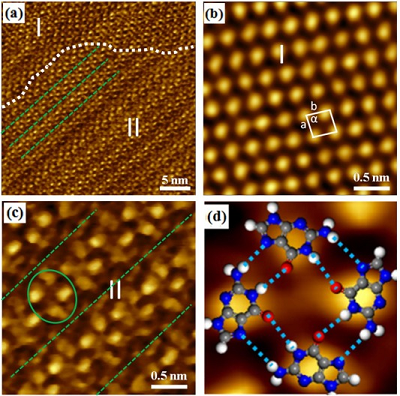
\includegraphics[width=\textwidth]{Chapter3/Figures/Figure6.png}
    \caption[Number density ($\eta$) for Cl\textsuperscript{-} as a function of the distance from topmost graphene sheet, from 1M additive and Drude polarizable FF salt simulations]{Number density ($\eta$) for  Cl\textsuperscript{-} as a function of the distance from topmost graphene sheet, from 1M additive and Drude polarizable FF salt simulations. All distances are presented in units of $\angstrom$.}
\end{figure}

The ion density distribution for the cations depends on both the size of the cation as well as the underlying FF. For all the systems we observe that the additive simulations favour the interactions between the solvated cation and the graphene sheet, with the major peak in the distribution being observed in the range between 5.7-7.7 $\angstrom$. We observe that this is being driven by the distribution of the counter ion Cl\textsuperscript{-} in the system which is observed at around $\approx$6.40 $\angstrom$ for all the systems. For Li\textsuperscript{+}, Na\textsuperscript{+}, Mg\textsuperscript{2+} and Ca\textsuperscript{2+} we also observe minor peaks in the distribution at 4.9 $\angstrom$, 4.8 $\angstrom$, 4.8 $\angstrom$ and 4.7 $\angstrom$, which correspond to the direct interaction of the ions with the graphene surface or the interaction of a partially solvated ion with the graphene surface. For Li\textsuperscript{+}, Na\textsuperscript{+}, Mg\textsuperscript{2+} and Ca\textsuperscript{2+} this interaction is favoured due to the favourable free energy associated with such interactions [Figure 5.2] in the additive FF. For the Drude polarizable FF we observe two distinct favourable interactions depending on the cations. Li\textsuperscript{+}, Mg\textsuperscript{2+} and Ca\textsuperscript{2+} favour a direct interaction between the cations or partially solvated cations and the graphene surface with the major peak in the distribution being observed at 4.0 $\angstrom$, 4.8 $\angstrom$ and 5.1 $\angstrom$, respectively. On the other hand, Na\textsuperscript{+}, K\textsuperscript{+} and Cs\textsuperscript{+} favour interaction between a fully solvated cation and the graphene surface, with the major peaks being observed at 7.7 $\angstrom$, 6.1 $\angstrom$ and 6.4 $\angstrom$ respectively. Interestingly for Ca\textsuperscript{2+} we observe the next peak in the distribution at 6.1 $\angstrom$. This close pacing of the peaks is correlated to the broad shallow minimum observed in the free energy profile for Ca\textsuperscript{2+} obtained using the Drude polarizable FF parameters [Figure 5.3]. The increased propensity of Li\textsuperscript{+}, Mg\textsuperscript{2+} and Ca\textsuperscript{2+} to reside close to the graphene surface in Drude polarizable FF simulations is also driven by the prominent density of Cl\textsuperscript{-} near the graphene surface with the Cl\textsuperscript{-} distribution being observed at 3.8 $\angstrom$. A decrease in the Cl\textsuperscript{-} ion density at 3.8 $\angstrom$, which is correlated to the peak height at 3.8 $\angstrom$ (Ca\textsuperscript{2+} > Mg\textsuperscript{2+} > Li\textsuperscript{+} $\approx$ Na\textsuperscript{+} > K\textsuperscript{+} > Cs\textsuperscript{+}) results in a shift in the Na\textsuperscript{+}, K\textsuperscript{+} and Cs\textsuperscript{+} densities away from the graphene surface.

\begin{figure}
    \centering
    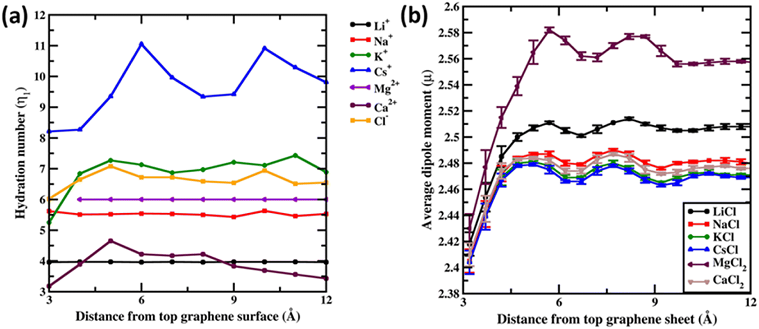
\includegraphics[width=\textwidth]{Chapter3/Figures/Figure7.png}
    \caption[First hydration number ($\eta_1$) for Li\textsuperscript{+}, Na\textsuperscript{+}, K\textsuperscript{+}, Cs\textsuperscript{+}, Mg\textsuperscript{2+}, Ca\textsuperscript{2+} and Cl\textsuperscript{-} ions from 1 M ion - graphene simulations as a function of distance from the graphene surface. Average dipole moment ($\mu$) for water molecules in various 1 M salt solutions discussed in the study are also presented]{(a) First hydration number ($\eta_1$) for Li\textsuperscript{+}, Na\textsuperscript{+}, K\textsuperscript{+}, Cs\textsuperscript{+}, Mg\textsuperscript{2+}, Ca\textsuperscript{2+} and Cl\textsuperscript{-} ions from 1 M ion - graphene simulations as a function of distance from the graphene surface. (b) Average dipole moment ($\mu$) for water molecules in various 1 M salt solutions discussed in the study. All distances are presented in units of $\angstrom$. Dipole moments are presented in units of Debye.}
\end{figure}

Before concluding we analyse the hydration dynamics of the water molecules around the ions from the Drude polarizable FF simulations. In Figure 5.7(a) we present the average hydration number computed for ions within blocks of 1 A as a function of distance from the graphene sheet. For the monovalent ions we observe that the hydration number increases as a function of the size of the ion. The average hydration number for Li\textsuperscript{+} and Na\textsuperscript{+} was found to be 3.96 and 5.62 irrespective of the distance from the graphene sheet indicative of a near tetra-coordinated and near hexa-coordinated structure for the first hydration shell in these systems. This is also observed in the representative structures presented in Figure 5.2. The larger monovalent ions K\textsuperscript{+} and Cs\textsuperscript{+} exhibit variable hydration numbers depending upon the distance from the graphene sheet. The K\textsuperscript{+} ions exhibit a distorted pentagonal bipyramidal geometry in the bulk with the hydration number being 6.92 for the first hydration shell. Closer to the graphene sheet the hydration number is found to be 5.25 indicating a loss of one/two water molecules from the bulk hepta-coordinated structure. For the largest ion Cs\textsuperscript{+} we observe variable hydration numbers in the bulk, with the hydration number varying from 9.21 to 11.05. This indicates an unstructured dynamic first hydration shell around Cs\textsuperscript{+}. Close to the graphene surface the hydration shell easily loses water molecules and the hydration number drops to 8.21. For the divalent ion Mg\textsuperscript{2+} the average hydration number was found to be 6.00 irrespective of the distance from the graphene sheet. However, a closer inspection of the structure of the hydration shell reveals that near the graphene sheet the hydration shell rearranges into a pentagonal pyramidal structure while in the bulk the hydration shell resembles an octahedral structure [Figure 5.3]. The larger divalent ion Ca\textsuperscript{2+} exhibits a variable hydration number like K\textsuperscript{+} and Cs\textsuperscript{+}. Close to the graphene sheet the hydration number is found to be 3.18, while in the bulk solution the hydration number was found to vary between 3.00 and 4.65. This points to a significant deviation from the octa-coordinated crystal environment for the Ca\textsuperscript{2+} ions in CaCl\textsubscript{2} salt. The hydration shell around Cl\textsuperscript{-} also undergoes partial reorganization upon interacting with the graphene surface. The hydration number drops to 6.02 from a bulk value of 6.65. Visualizing the hydration shell structure reveals a pentagonal pyramidal arrangement of water molecules around Cl\textsuperscript{-} similar to the arrangement observed for Mg\textsuperscript{2+} [Figure 5.3].

Finally, we analyse the dipole moment of the water molecules as a function of the distance from the graphene surface. In Figure 5.7(b) we present the average dipole moment computed for water molecules within blocks of 0.5 $\angstrom$ as a function of distance from the graphene sheet. We note that, from additive FF simulations, the dipole moment of water molecules is constrained to be 2.374 D due to the rigid water model used in the simulations. However, the SWM4 water model used in the Drude polarizable FF simulations is able to respond to the changes in the local environment. Very close to the graphene sheet the average dipole moment of water molecules stabilizes at around 2.41 D, wherein the water molecules are in close contact with the hydrophobic graphene and the influence of ions is not felt. Moving away from the graphene sheet we begin to observe an increase in the ion densities of both the anions and the cations [Figure 5.4]. For MgCl\textsubscript{2} and LiCl simulations, we observe a significant change in the average dipole moment of water with the dipole moment increasing to 2.58 D and 2.51 D at a distance of 5.7 $\angstrom$ from the graphene sheet. This is due to the small size of Mg\textsuperscript{2+} (0.70 $\angstrom$) and Li\textsuperscript{+} (0.71 $\angstrom$) ions, which favours a large charge/surface area ratio resulting in significant polarization of the local environment. On the other hand, for the larger cations we observe a reduced impact of the ions on the average dipole moment of water.

To comment on ion - graphene interactions and how the charges on the ions and the graphene surface respond to such interactions we analyse the dipole moment fluctuations for both the ions and the interacting graphene surface. In Figure C.1 of the Appendix C we present the instantaneous dipole moment of the ions as a function of distance from the graphene surface. In Figure C.2 of the Appendix C we present the instantaneous dipole moment of the interacting graphene surface as a function of distance from the ions. The instantaneous dipole moments of the ions [Figure C.1] and interacting graphene surface [Figure C.2] are found to be invariant with respect to the distance between the ions and the graphene surface. This indicates an absence of direct interaction between the ions and the graphene surface. This is highlighted in the observed distribution of the instantaneous dipole moment of the graphene sheet [Figure C.2], which appears independent of the chemical nature of the ions. However for both the ions and the graphene sheet we observe a spread in the dipole distribution. For the ions [Figure C.1] we observe a strong correlation between the distribution of the instantaneous dipole moments and the charge to surface ratio of the ions, with small ions such as Li\textsuperscript{+} and Mg\textsuperscript{2+} exhibiting a very small dipole distribution and larger ions such as Cs\textsuperscript{+} and Ca\textsuperscript{2+} exhibiting a broader distribution. This distribution can be traced back to the ion - water interactions in the first solvation shell of the ions. For the graphene sheet we observe a distribution from 0.0 D to 2.4 D [Figure C.2]. This dipole response of the graphene surface can be traced back to the interactions with the water molecules present in the 1\textsuperscript{st} monolayer of water observed at 3.40 $\angstrom$ [Figure 5.5]. Thus, we only observe solvent driven interactions between the ions and the graphene surface.
\section{Conclusions}
In conclusion, we show that the Drude polarizable FF parameters for graphene\supercite{h_polarization_2021} along with the parameters for ions\supercite{yu_simulating_2010} reliably capture the dynamics at the graphene electrolyte interface. The Drude parameters are able to capture both the size and charge dependent ion - graphene interactions, which cannot be captured by additive simulations. In particular the Drude parameters are able to capture the anion - graphene interactions, which are severely underestimated in the additive simulations. Additionally, the Drude polarizable simulations also capture the influence of ions on solvation dynamics. These results establish the applicability of Drude parameters for studying ion - graphene interface interactions, like those observed in graphene-based membranes for desalination,\supercite{sun_selective_2014,joshi_precise_2014,homaeigohar_graphene_2017,boretti_outlook_2018,yang_ultrathin_2017} or graphene-based electrodes in energy storage.\supercite{liang_graphene-based_2009,wang_supercapacitor_2009,wang_sngraphene_2009,stoller_graphene-based_2008} The Drude parameters also present an effective alternative to computationally expensive first-principles MD simulations.